\documentclass[8pt,pdf,hyperref={unicode}]{beamer}
% \documentclass[aspectratio=43]{beamer}
% \documentclass[aspectratio=1610]{beamer}
% \documentclass[aspectratio=169]{beamer}
\usepackage{lmodern}
\usepackage{amsfonts}
\usepackage{amsmath}
\usepackage{listings}
\usepackage{mwe,tikz}
% тема оформления
%\usetheme{CambridgeUS}
%Закругление выделений
%\useinnertheme{rounded}
%Настройка темы самого слайда
%\useoutertheme{infolines}
%\useoutertheme[subsection=true, footline=authortitle]{miniframes}
\usetheme{Boadilla}
\useoutertheme[subsection=true, footline=authortitle]{miniframes}
\makeatother
\setbeamertemplate{footline}
{
    \leavevmode%
    \hbox{%
        \begin{beamercolorbox}[wd=.4\paperwidth,ht=2.25ex,dp=1ex,center]{author in head/foot}%
            \usebeamerfont{author in head/foot}\insertshortauthor
        \end{beamercolorbox}%
        \begin{beamercolorbox}[wd=.6\paperwidth,ht=2.25ex,dp=1ex,center]{title in head/foot}%
            \usebeamerfont{title in head/foot}\insertshorttitle\hspace*{3em}
            \insertframenumber{} / \inserttotalframenumber\hspace*{1ex}
        \end{beamercolorbox}}%
        \vskip0pt%
    }
\makeatletter
% отключить клавиши навигации
\setbeamertemplate{navigation symbols}{}
% цветовая схема
\usecolortheme{spruce}


\title[BM@N NICA Condition database]{Development of services for the condition database of the BM@N experiment at NICA}   
%\subtitle{Overview report}
\author{\underline{Mikhail Zelenyi}\inst{1,2} \and  Peter Klimai\inst{1,2} \and  Konstantin Gertsenberger\inst{3}}
\institute[INR]{
    \inst{1} Institute for Nuclear Research RAS \and
    \inst{2} Moscow Institute of Physics and Technology \and
    \inst{3} Joint Institute for Nuclear Research
    }
\date{\today}

%\logo{\includegraphics[height=5mm]{image/logo.png}\vspace{-7pt}}

\begin{document}
% титульный слайд
\begin{frame}
 \titlepage
\end{frame}

\begin{frame}
	\frametitle{NICA Megaproject}
	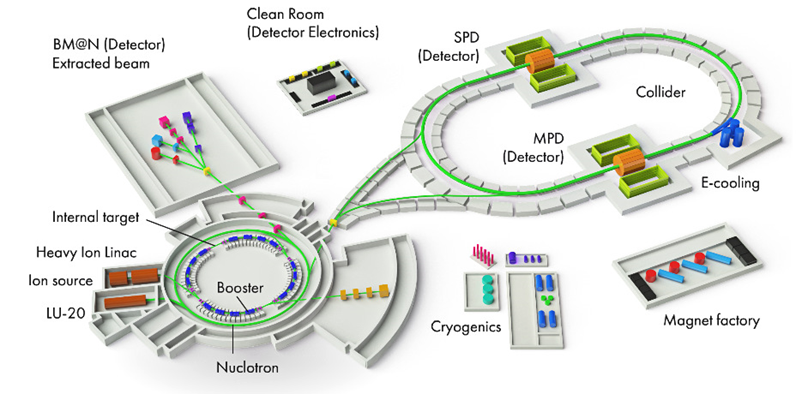
\includegraphics[width=\linewidth]{image/slide1.png}
\end{frame}
\begin{frame}
	\frametitle{BM@N Software-Computing Architecture (design)}
	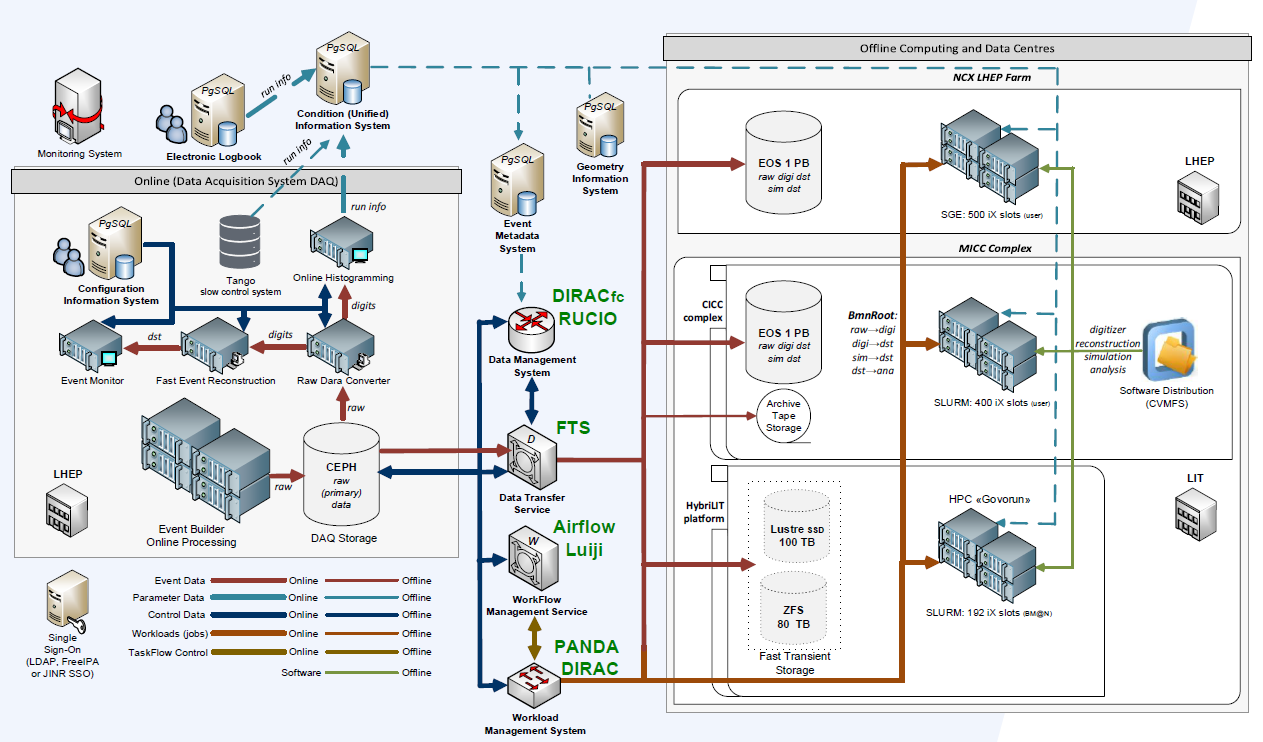
\includegraphics[width=\linewidth]{image/slide2.png}
\end{frame}
\begin{frame}
	\frametitle{BM@N Condition Database Schema}
	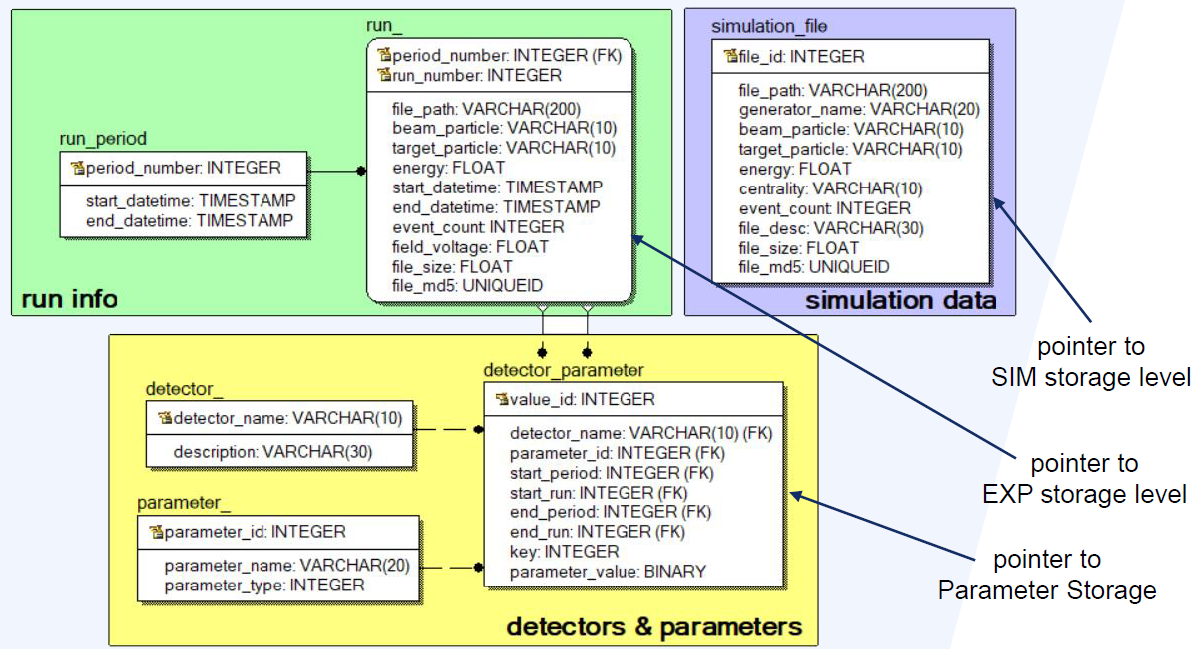
\includegraphics[width=\linewidth]{image/slide3.png}
\end{frame}

\begin{frame}
	\frametitle{Services for Condition Database}
	\begin{columns}
		\begin{column}{0.5\linewidth}
			C++ API
			\begin{itemize}
				\item Autogenerated class wrappers for database tables with specific functions allow to access and manage data in the BmnRoot framework
			\end{itemize}
			REST API
			\begin{itemize}
				\item Modern interface for integration with other software components
			\end{itemize}
			Web UI by Alexander Chebotov
			\begin{itemize}
				\item Visualization of summary data in the form of diagrams and charts
				\item Convenient viewing, managing and searching for up-to-date information on the BM@N experiment in tabular view by collaboration members
			\end{itemize}
			Service scripts
			\begin{itemize}
				\item Auto updating simulation file list
				\item Checking integrity of the raw data files
			\end{itemize}
		\end{column}
		\begin{column}{0.5\linewidth}
			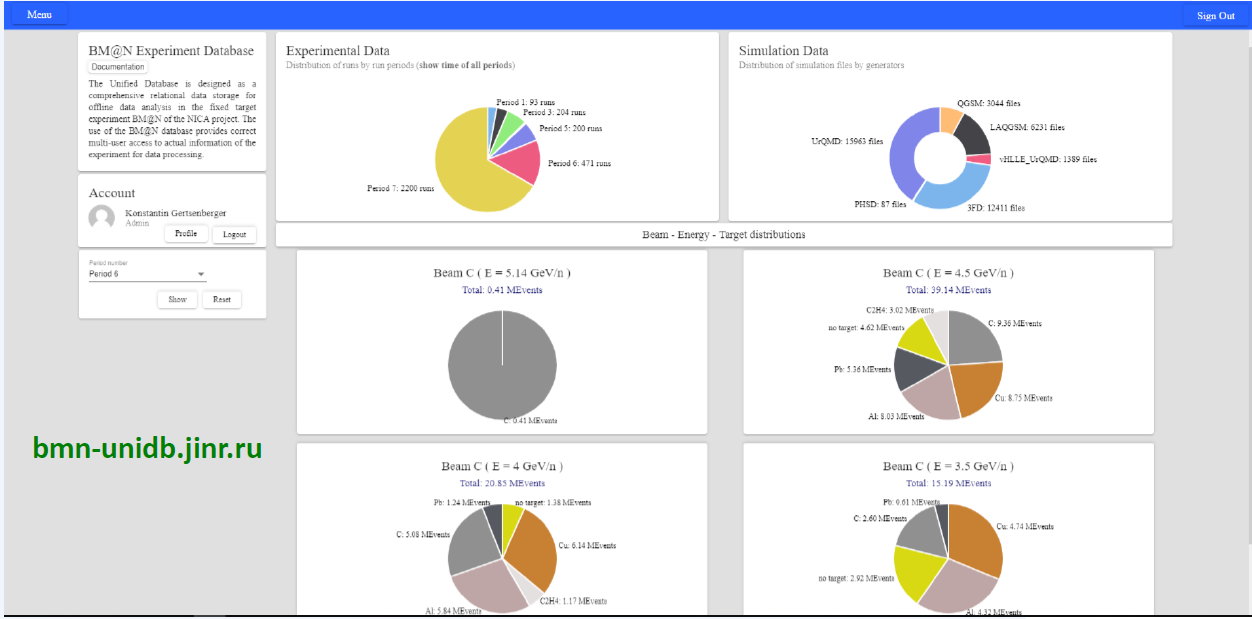
\includegraphics[width=\linewidth]{image/slide4.png}
		\end{column}
	\end{columns}
\end{frame}
\begin{frame}
	\frametitle{Smart Data Parser}
	\begin{columns}
		\begin{column}{0.5\linewidth}
			\begin{itemize}
				\item Smart Data Parser --- utile for transfer text data to database
				\item Using data model defined in JSON format
				\item Working with different formats (CSV and XML in now)
				\item Working with different database (PostgresSQL on NICA)
				\item Implement by Python, have CLI and Qt-based GUI. 
			\end{itemize}
		\end{column}
		\begin{column}{0.6\linewidth}
			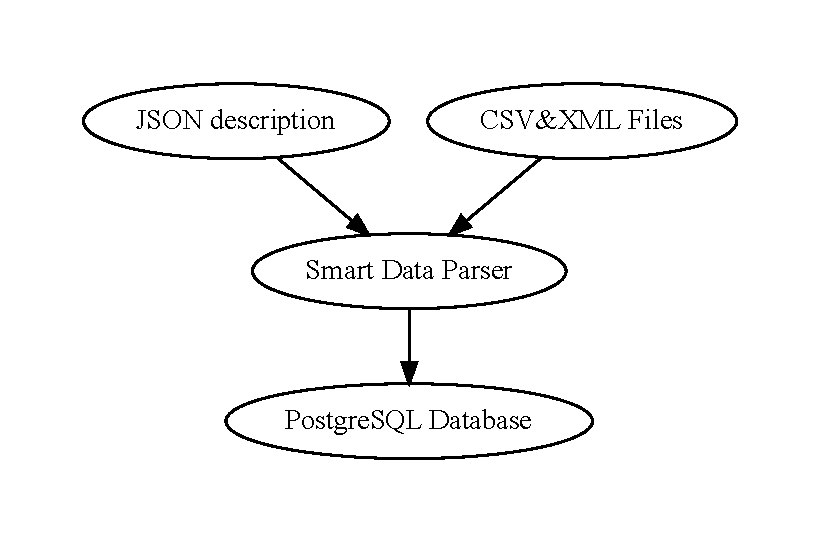
\includegraphics[width=\linewidth]{image/schema_1.dot.pdf}
		\end{column}
	\end{columns}
\end{frame}

\begin{frame}
    \frametitle{Smart Data Parser: Database communication}
	\begin{columns}
	\begin{column}{0.5\linewidth}
		\begin{itemize}
				\item Python Database API 2.0 (PDAPI 2.0)\footnotemark --- specification for unification API for connectors to different database
				\item SqlAlchemy\footnotemark --- framework for safe generation SQL for PDAPI 2.0, database communication and Object-Relation Mapping
				\item Communication with database metadata allows validating JSON data descriptions or create templates using information about columns names and types
				
		\end{itemize}

	\end{column}
	\begin{column}{0.5\linewidth}
		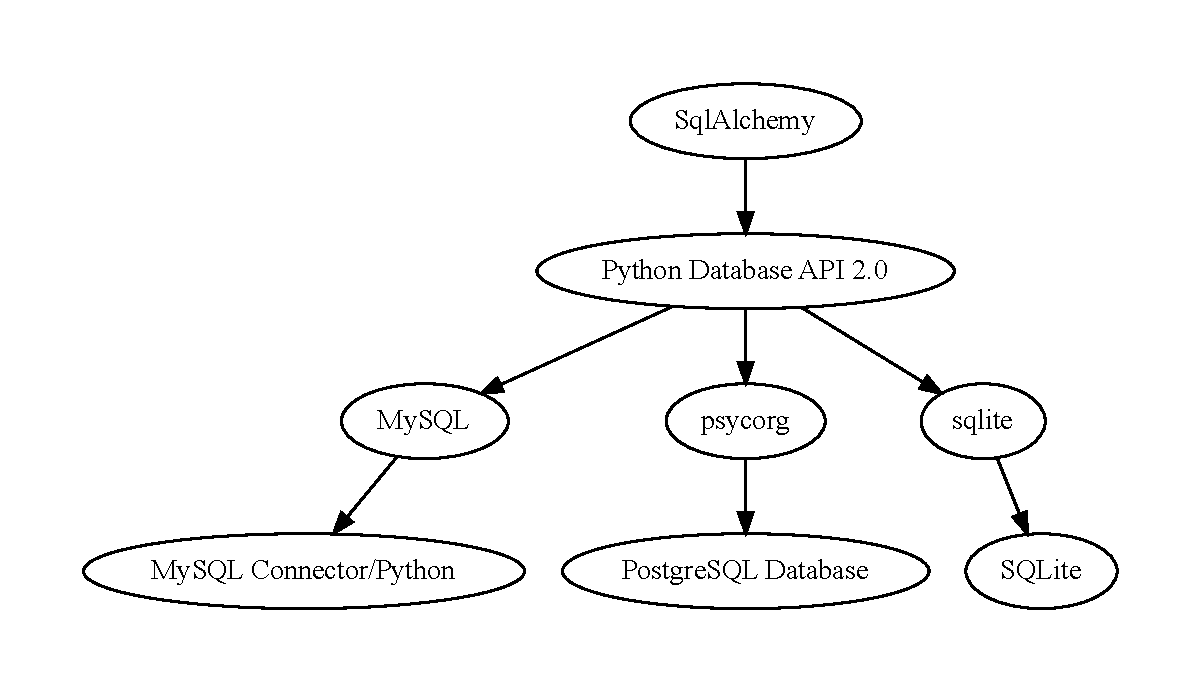
\includegraphics[width=\linewidth]{image/schema_2.dot.pdf}
	\end{column}
	\end{columns} 
	\footnotetext[1]{\href{https://peps.python.org/pep-0249/}{https://peps.python.org/pep-0249/}}
	\footnotetext[2]{\href{https://www.sqlalchemy.org/}{https://www.sqlalchemy.org/}}
\end{frame}

\begin{frame}
	\frametitle{Smart Data Parser: Data descriptions}
	\begin{columns}
		\begin{column}{0.5\linewidth}
			JSON descriptions allow describe:
			\begin{itemize}
				\item Target table in database
				\item Options fo data file parser
				\item Structure of data file and relationships between data and columns of database table
			\end{itemize}
			JSON Schema\footnotemark of JSON descriptions
			\begin{itemize}
				\item Validate  JSON descriptions with \texttt{jsonschema}\footnotemark
				\item Generate documentation in HTML an Markdown with \texttt{json-schema-for-humans}\footnotemark
				\item Define default values
			\end{itemize}

		\end{column}
		\begin{column}{0.5\linewidth}
			\lstinputlisting{temp.json}
		\end{column}
	\end{columns} 
	\footnotetext[3]{\href{https://json-schema.org/}{https://json-schema.org/}}
	\footnotetext[4]{\href{https://github.com/python-jsonschema/jsonschema}{https://github.com/python-jsonschema/jsonschema}}
	\footnotetext[5]{\href{https://coveooss.github.io/json-schema-for-humans/\#/}{https://coveooss.github.io/json-schema-for-humans/\#/}}
\end{frame}


\begin{frame}
	\frametitle{Smart Data Parser: CLI Usage : Generation}
	\vspace{-2.5em}
		\begin{columns}
				\begin{column}{0.65\linewidth}
					\begin{block}{Database}
						\lstinputlisting[basicstyle=\small]{shell/shell1.txt}
					\end{block}
					\end{column}
				\begin{column}{0.35\linewidth}
				\begin{block}{detector\_.json}
					\lstinputlisting[basicstyle=\small]{shell/detector_.json}
				\end{block}
					\end{column}
			\end{columns} 
		\begin{block}{Run generation}
			\lstinputlisting{shell/shell2.txt}
		\end{block}
\end{frame}

\begin{frame}
	\frametitle{Smart Data Parser: CLI Usage: Loading}
		\vspace{-3em}
		\lstinputlisting{shell/shell3.txt}
		\begin{columns}
			\begin{column}{0.35\linewidth}
				\begin{block}{detector\_.json}
					\lstinputlisting[basicstyle=\small]{shell/detector_.json}
				\end{block}

			\end{column}
			\begin{column}{0.15\linewidth}
				\begin{block}{detector\_.csv}
					\lstinputlisting[basicstyle=\small]{shell/detector_.csv}
				\end{block}
				
			\end{column}
			\begin{column}{0.4\linewidth}
				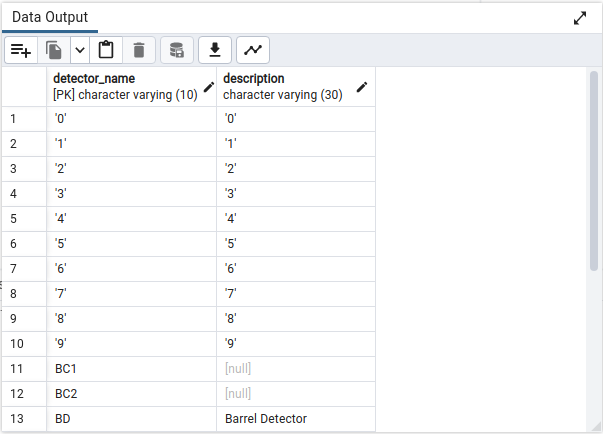
\includegraphics[width=\linewidth]{image/pgadmin.png}
			\end{column}
		\end{columns} 
\end{frame}

\begin{frame}
	\frametitle{Smart Data Parser: GUI}
	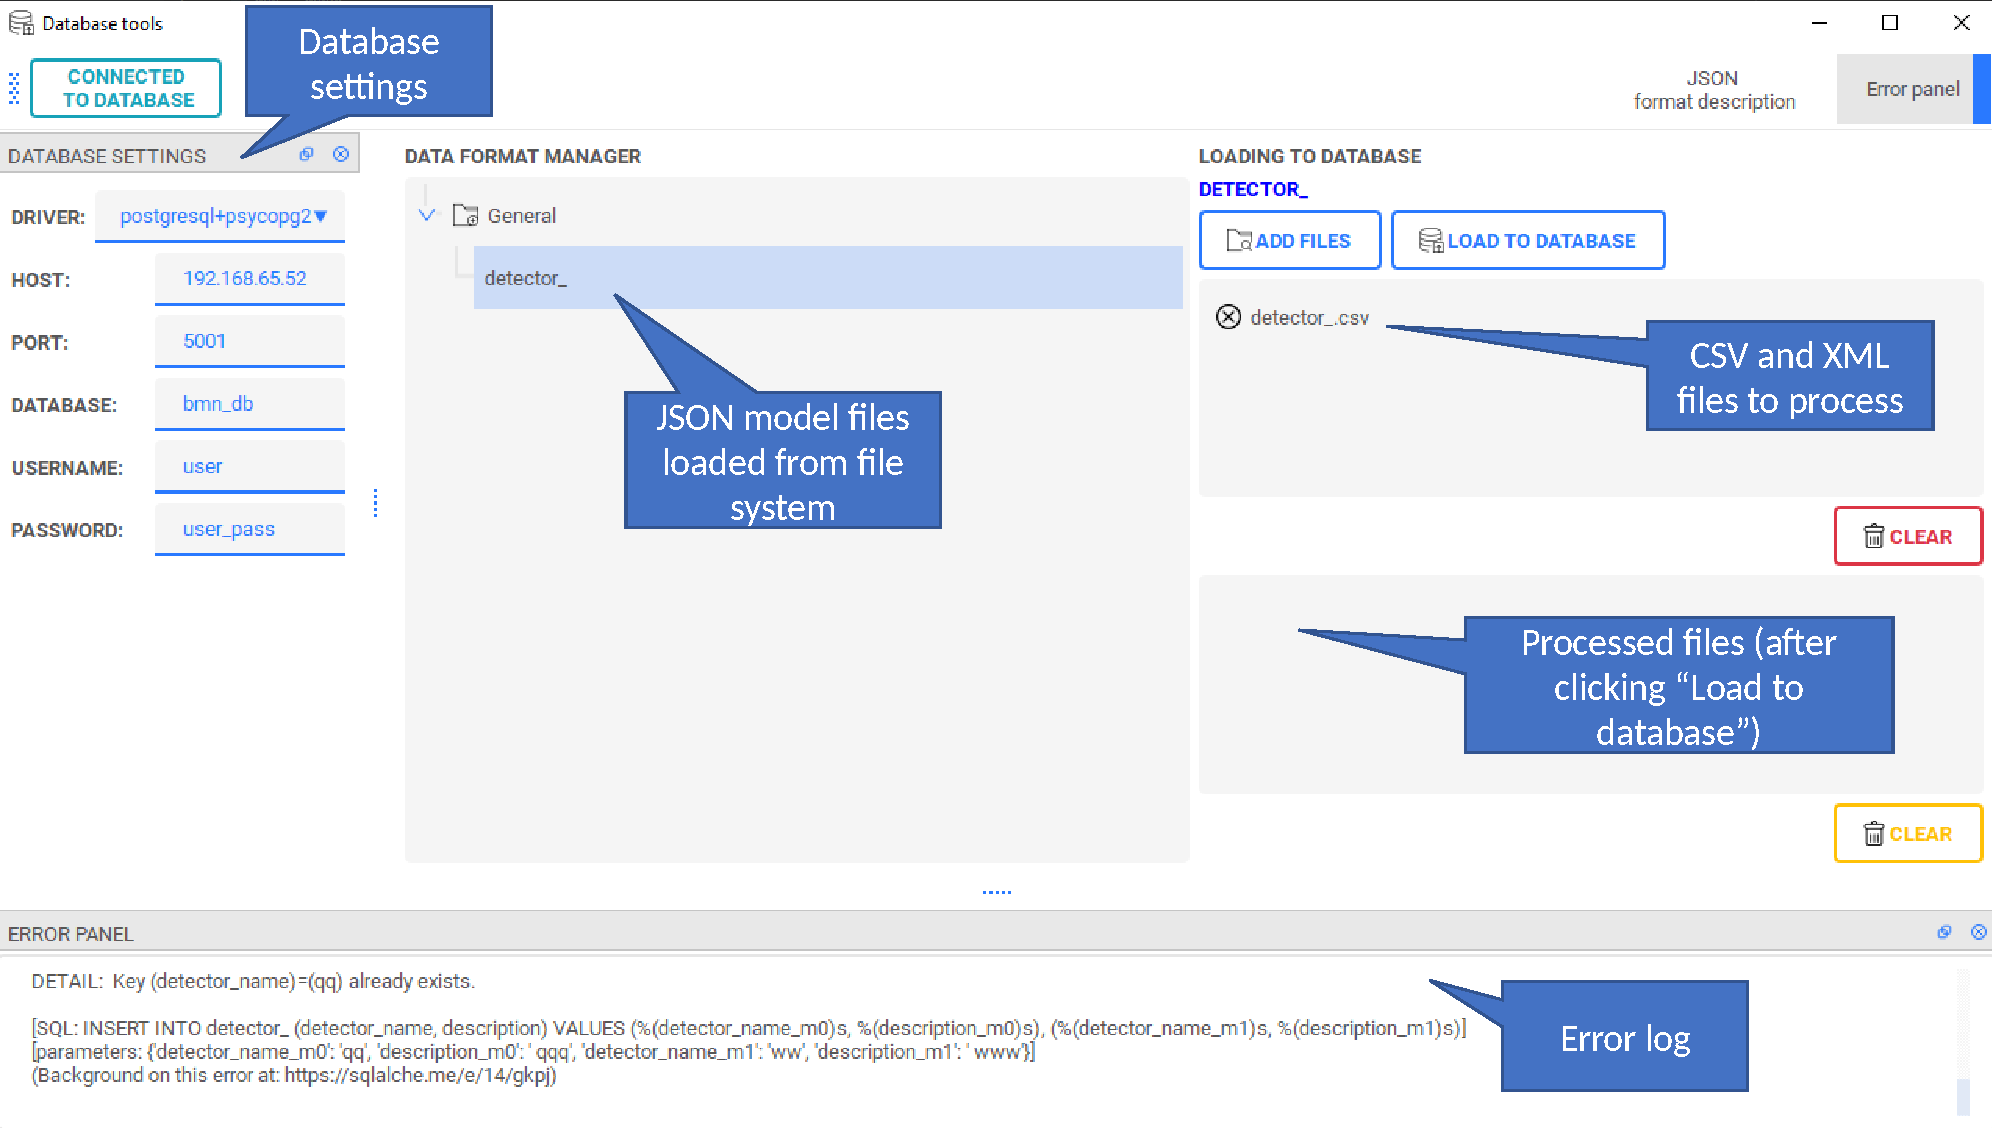
\includegraphics[width=\linewidth]{image/gui.pdf}
\end{frame}


\begin{frame}
	\frametitle{Smart Data Parser: GUI development}
	\begin{columns}
		\begin{column}{0.5\linewidth}
			For GUI used PySide\footnotemark --- Python Qt binding
			\begin{itemize}
				\item Using PySide2 with Qt5, can be run with Qt6
				\item For material design used \texttt{qt-material}\footnotemark 
			\end{itemize}
			JSON schema:
			\begin{itemize}
				\item Using for autogenerating description editor
			\end{itemize}
		\end{column}

		\begin{column}{0.5\linewidth}
		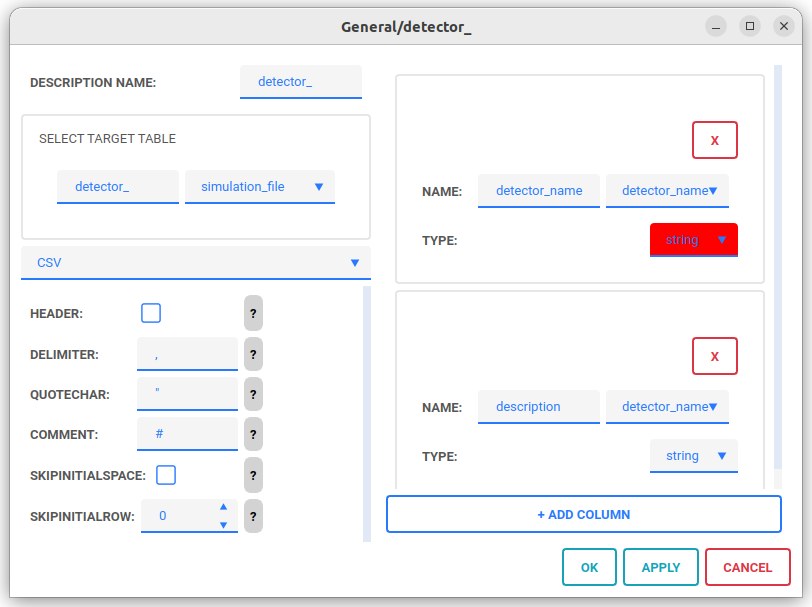
\includegraphics[width=\linewidth]{image/gui2.png}
		\end{column}
	\end{columns}
	\footnotetext[6]{\href{https://www.qt.io/qt-for-python}{https://www.qt.io/qt-for-python}}
	\footnotetext[7]{\href{https://pypi.org/project/qt-material/}{https://pypi.org/project/qt-material/}}
\end{frame}
\begin{frame}
	\frametitle{Thank you for your attention}

	
\includegraphics[width=\linewidth]{image/python.png}

\end{frame}

\end{document}